\newcommand{\env}[1]{\texttt{#1}}
\newcommand{\command}[1]{\texttt{#1}}
\newcommand{\package}[1]{\texttt{\itshape#1}}
\newcommand{\engl}[1]{(engl: \textit{#1})\xspace}
\setlength{\parindent}{0pt}
\lstset{extendedchars=\true}
\lstset{inputencoding=ansinew}
\newcommand\tab[1][1cm]{\hspace*{#1}}
\newpage

\section{Aufgabe 1 - Firewall mit IPTables}

\subsection{Teilaufgabe a)}

\subsubsection{Frage- bzw. Aufgabenstellung}

Welche Ports verwenden die Programme zur Kommunikation? Wie ändert man die Standardeinstellungen? Ist dazu ein Neustart des Systems nötig?

\subsubsection{Lösung}

Bei Linux Betriebssystemen kann man sich  die verwendeten Ports mit dem Befehl \textit{netstat -tulpn} anzeigen lassen. netstat ist ein häufig benutztes Diagnose-Werkzeug um verschiedene Informationen über die Netzwerkschnittstellen anzeigen zu lassen. Die Portnummer sieht man dann in der Spalte \textit{Local Address} nach dem letzten Doppelpunkt. Dies sollte dann so aussehen: 

\begin{figure}[htbp]
\begin{center}
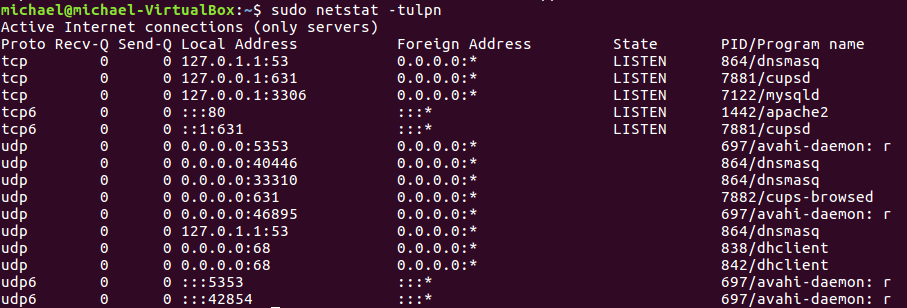
\includegraphics[width=0.7\textwidth]{Bild1}
\caption{Portnummer anzeigen lassen}
\end{center}
\end{figure}

\subsubsection{Ergebnis}

Wir können die verschiedenen Ports der Programme auslesen.

\subsection{Teilaufgabe b)}

\subsubsection{Frage- bzw. Aufgabenstellung}

Richten Sie eine restriktive Firewall ein (prohibitive Sicherheitspolitik). Es soll sichergestellt werden, dass ausschließlich der Port des Webservers von außen zugänglich ist. Die Firewall soll automatisch beim Start des Systems geladen werden. Nutzen Sie für die Lösung der Aufgabe ausschließlich die Kommandozeile und das Kommando iptables.

\subsubsection{Lösung}

Da der Webserver den Port 80 (localhost) besitzt, müssen wir dafür sorgen, dass nur eingehende Pakete für diesen Port angenommen werden und sonst keine. Dafür benutzen wir den Befehl \textit{iptables -A INPUT -i lo -j ACCEPT}. Das -A hängt eine Regel an die \textit{Chain} an, dass -i ist für die Netzwerkschnittstelle zuständig über die Pakete eingehen (in diesem Fall localhost) und das -j legt die Aktion fest. Anschließend benutzen wir noch den Befehl \textit{iptables -A INPUT -j DROP} damit keine weiteren Pakete angenommen werden. Daher auch der Command \textit{DROP}. Diese Befehle schreiben wir in eine neue Datei im init.d Ordner.
\textit{touch /etc/init.d/firewall && chmod 755 /etc/init.d/firewall && nano /etc/init.d/firewall}. Damit das Skript bei jedem Neustart ausgeführt wird, schreiben wir folgenden Code in die \textit{rc.local}-Datei:

\begin{lstlisting}[caption={rc.local}]
if [ -e '/etc/init.d/firewall' ]
then
    /bin/sh '/etc/init.d/firewall'
fi
\end{lstlisting}

\subsubsection{Ergebnis}

Wir können mit \textit{iptables} eine Firewall einstellen und sorgen dafür, dass die Firewall bei jedem Systemstart aktiv ist.

\subsection{Teilaufgabe c)}

\subsubsection{Frage- bzw. Aufgabenstellung}


\subsubsection{Lösung}


\subsection{Teilaufgabe d)}

\subsubsection{Frage- bzw. Aufgabenstellung}

Nun öffnen Sie mit netcat auf dem Rechner A (eine Ihrer VMs) ein oder zwei Ports zwischen 0 und 100. Nutzen Sie dafür den Befehl: nc -l [Portnummer].\\
\\
nmap ist ein Portscanner, mit dem man u.a. die eigene Firewall auf Sicherheitslücken testen kann. Mit \\
nmap Zieladresse -p [Anfangsport]-[Endport] \\
kann nach offenen Ports in einem bestimmten Portbereich gescannt werden. Führen Sie nun einen Portscan auf VM A von VM B aus. Welches Ergebnis sehen Sie?

\subsubsection{Lösung}

Zunächst öffnen wir den Port 48 mit dem Befehl \textit{nc -l 48}. Anschließend scannen wir den Port mit dem Befehl \textit{nmap localhost -p 48}. Wie man in Abbildung ~\ref{fig:Portscan} erkennen kann, bekommt man die Ausgabe dass der Port offen ist (STATE -> open). Wenn ich nun von einer anderen VM einen Portscan ausführe, wird auch hier erkannt dass der Port mit der Nummer 48 auf der VM A offen ist (siehe Abbildung ~\ref{fig:Portscan2}). 

\begin{figure}[htbp]
\begin{center}
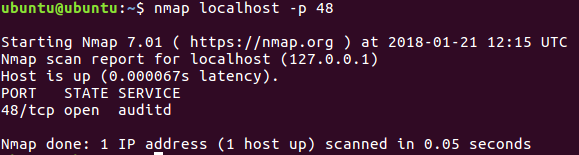
\includegraphics[width=0.7\textwidth]{Bild2}
\caption{Portscan mit nmap}
\label{fig:Portscan}
\end{center}
\end{figure}

\begin{figure}[htbp]
\begin{center}
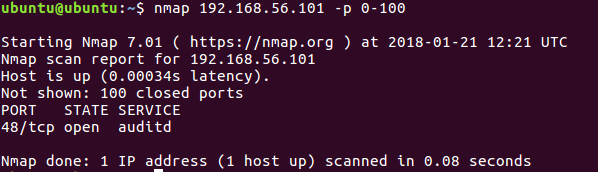
\includegraphics[width=0.7\textwidth]{Bild3}
\caption{Portscan von anderer VM}
\label{fig:Portscan2}
\end{center}
\end{figure}

\subsubsection{Ergebnis}

Wir können mit dem Befehl netcat verschiedene Ports öffnen und nmap anwenden um einen Portscan durchzuführen.

\subsection{Teilaufgabe e)}

\subsubsection{Frage- bzw. Aufgabenstellung}

Definieren Sie nun Regeln mit iptables, die einen solchen Scan blocken. Dazu bietet es sich an, alle Pakete zu verwerfen, die ungewöhnlich schnell Verbindungsanfragen senden. \\
Sehen Sie sich die folgende Regel an und versuchen Sie zu verstehen, welchen Sinn einzelne Befehle erfüllen. Sie werden sie im Verlauf dieser Übung noch benötigen

\subsubsection{Lösung}

Die Regel \textit{iptables -A INPUT -p tcp -i eth1 -m state --state NEW -m recent --set} sagt zunächst am Anfang, dass es sich um eine Regel handelt die eine neue Chain vom Typ INPUT anhängt (-A INPUT). Des weiteren wird mit dem Befehl \textit{-p} gesagt, dass nur Pakete vom Protokoll tcp überprüft werden und die \textit{-i} Option sagt aus, dass nur Pakete von der Netzwerkschnittstelle \textit{eth1} überprüft werden. Weiterhin wird noch gesagt, dass nur Pakete mit dem Status \textit{NEW} überprüft werden. \textit{recent} erlaubt es dynamisch Listen mit IP-Adressen zu erstellen und dann an Hand der Listen Pakete zu filtern.


\subsubsection{Ergebnis}

Wir können die aufgezeichneten Pakete analysieren und wissen warum eine DNS-Abfrage für den HTTP-Nachrichtenaustausch erforderlich ist.


\subsection{Teilaufgabe g)}

\subsubsection{Frage- bzw. Aufgabenstellung}

Auf Ebene der IP-Kommunikation wird im IP-Header gespeichert, welches Protokoll auf der darüber liegenden Transportschicht verwendet wird. Wie heißt das Feld im IP-Header, in dem diese Information gespeichert wird? Welche Nummer hat das für DNS genutzte Transportprotokoll UDP und welche Nummer hat TCP?


\subsubsection{Lösung}

Das Protokoll wird im Feld \textit{Protocol} gespeichert welches 8 Bit groß ist. Den Aufbau des IP-Headers sieht man in Abbildung 7.\cite{[1]} UDP hat die Protokollnummer 17, während TCP die Nummer 6 besitzt.\cite{[2]}

\begin{figure}[htbp]
\begin{center}
\includegraphics[width=0.7\textwidth]{Bild8}
\caption{IP-Header}
\end{center}
\end{figure}

\subsubsection{Ergebnis}

Wir kennen uns mit dem IP-Header aus und kennen die Protokollnummern für UDP und TCP.


\section{Aufgabe 3 - Protokolle auf Netzwerkebene überwachen}

\subsection{Teilaufgabe b)}

\subsubsection{Frage- bzw. Aufgabenstellung}

Sehen Sie sich mit dem Kommando arp -a den Inhalt des ARP-Caches Ihres Rechners an. Stellen Sie sicher, dass der Cache leer ist.

\subsubsection{Lösung}

Zunächst löschen wir den Cache mit \textit{arp -d} und lassen uns danach den Cache mit \textit{arp -a} anzeigen. Das ganze sieht dann so aus:

\begin{figure}[htbp]
\begin{center}
\includegraphics[width=0.7\textwidth]{Bild9}
\caption{ARP-Cache}
\label{fig:ARP-Cache}
\end{center}
\end{figure}

\subsubsection{Ergebnis}

Wir können uns den ARP-Cache anzeigen lassen.

\subsection{Teilaufgabe c)}

\subsubsection{Frage- bzw. Aufgabenstellung}

Starten Sie den Wireshark und stellen Sie nun in einen neuen Capture-Filter mit dem Namen und ARP und dem Filter-String arp or icmp ein und starten Sie ein neues Capturing. Führen Sie dann einen Ping (ping -c 1) auf einen Rechner in Ihrem lokalen Netz aus. Betrachten Sie die ersten beiden Frames und tragen Sie die folgenden Informationen in die Tabelle ein. Um welche Art von Frames handelt es sich hier?

\subsubsection{Lösung}

Zunächst stellen wir den Capture-Filter \textit{arp or icmp} ein, wie wir es auch schon in Aufgabe 2 gemacht haben und starten die Aufzeichnung. Nun geben wir in der Kommandozeile den Befehl \textit{ping -c <IP-Adresse>} ein und beobachten die Aufzeichnung. Die Informationen sehen sie in der folgenden Tabelle. Es handelt sich in diesem Fall um ARP Frames.

\begin{figure}[htbp]
\begin{center}
\includegraphics[width=0.8\textwidth]{Bild10}
\caption{ARP Aufzeichnungen}
\end{center}
\end{figure}

\subsubsection{Ergebnis}

Wir können ARP Protokolle aufzeichnen und auswerten.

\subsection{Teilaufgabe d)}

\subsubsection{Frage- bzw. Aufgabenstellung}

Überprüfen Sie mit dem Kommando arp -a den Inhalt des ARP-Caches Ihres Rechners. Welche MAC-Adresse besitzt der Webserver?

\subsubsection{Lösung}

Wie man in Abbildung ~\ref{fig:ARP-Cache} sehen kann, hat der Webserver die MAC-Adresse \textit{01:00:5e:00:00:16}.

\subsubsection{Ergebnis}

Wir können aus dem ARP-Cache die MAC-Adresse auslesen.


\section{Quellen}
\begin{thebibliography}{999}
\bibitem {1} Enrico Lauterschlag, Das Internet Protocol – Das Internet – Teil 6 \\ \url{http://www.webschmoeker.de/grundlagen/internet-protocol/#der_ip-header}, 16.01.2018 \\
\\
\bibitem {2} Robert W. Scheifler, Protocol Numbers \\ \url{https://www.iana.org/assignments/protocol-numbers/protocol-numbers.xhtml}, 16.01.2018

\end{thebibliography}




